
%(BEGIN_QUESTION)
% Copyright 2010, Tony R. Kuphaldt, released under the Creative Commons Attribution License (v 1.0)
% This means you may do almost anything with this work of mine, so long as you give me proper credit

For each of these FOUNDATION Fieldbus final control elements (valve positioner and variable-frequency motor drive), explain what the {\tt BKCAL\_OUT} signal from the respective AO function blocks represent:

$$\includegraphics[width=15.5cm]{i04579x01.eps}$$

Furthermore, identify how a FOUNDATION Fieldbus AO function block responds differently in {\it Cascade}, {\it Auto}, and {\it Manual} modes.

\vskip 20pt \vbox{\hrule \hbox{\strut \vrule{} {\bf Suggestions for Socratic discussion} \vrule} \hrule}

\begin{itemize}
\item{} In each example, identify a circumstance which could cause the ``back calculation'' signal value to not equal the input signal value.
\item{} FOUNDATION Fieldbus AO function blocks support the ability to limit the rate-of-change of an AO block's ``setpoint'' value.  Explain how this feature might be useful in either of these (valve, motor) control applications.
\end{itemize}

\underbar{file i04579}
%(END_QUESTION)





%(BEGIN_ANSWER)

For the valve positioner, the {\tt BKCAL\_OUT} signal represents actual valve stem position (assuming the positioner has a feedback mechanism to sense valve position).  Otherwise, this signal based on the {\tt OUT} value representing air pressure applied to the valve actuator.

\vskip 10pt

For the motor drive, the {\tt BKCAL\_OUT} signal represents actual motor speed (assuming the drive has speed feedback from the motor).   Otherwise, this signal based on the {\tt OUT} value representing the frequency of power applied to the motor.  

\vskip 10pt

In {\it Cascade} mode, the AO function block follows the value of the signal sent to it through its CAS\_IN input (from another FF function block).  In {\it Auto} mode, the AO block holds steady at a setpoint value entered manually into the block.  In {\it Manual} mode, the AO block outputs a fixed value and ignores the setpoint value.


%(END_ANSWER)





%(BEGIN_NOTES)


%INDEX% Fieldbus, function block: "back_cal" signal for a valve positioner
%INDEX% Fieldbus, function block: "back_cal" signal for a variable-frequency motor drive

%(END_NOTES)

